\titleformat{\chapter}[display]
  {\normalfont\bfseries}{}{0pt}{\Large} % Este comando es para eliminar la aparición de "Capítulo N" en el PDF. Para emplear el formato de la tesis simplemente eliminamos la línea. 
\chapter{Planteamiento del Problema}
\justifying
El dengue sigue siendo un problema de salud pública sin antivirales específicos realmente eficaces. La proteasa NS2B-NS3 del DENV-2 es un blanco terapéutico clave y los fulerenos funcionalizados con aminoácidos son plataformas prometedoras al mejorar su solubilidad y estructura electrónica. Aún se desconoce cómo estas modificaciones afectan su interacción con NS2B-NS3, por lo que estudiarlas puede aportar bases para diseñar nuevos inhibidores contra el dengue.
\begin{center}
\fcolorbox{AzulOscuro!30}{GrisClaro}{
            \begin{minipage}{0.9\textwidth}
                \small
               ¿Cómo afecta la funcionalización de fulerenos con aminoácidos a su estructura electrónica y qué impacto tiene en su interacción con la proteína del dengue NS2B-NS3 correspondiente al serotipo DENV-2?
            \end{minipage}
        }
  \end{center}
  
\begin{center}
  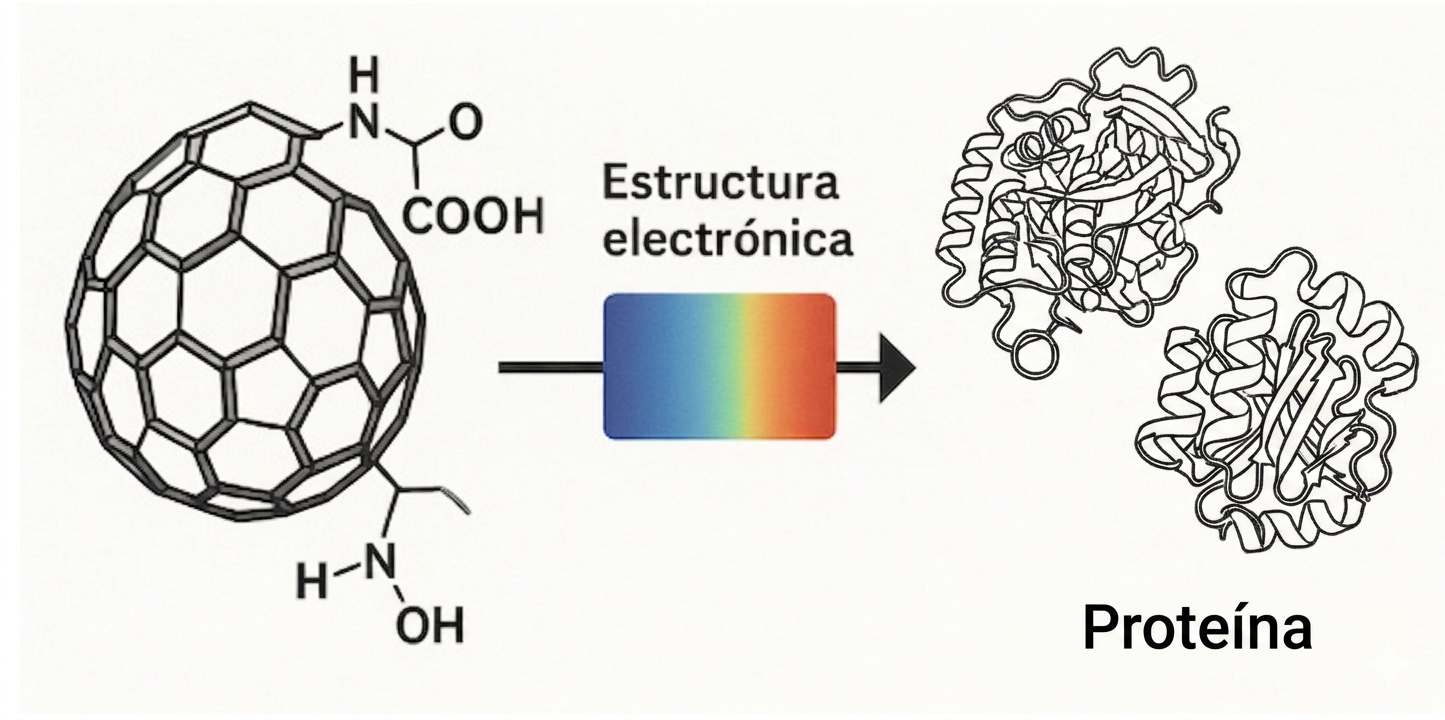
\includegraphics[width=0.6\textwidth,height=0.3\textwidth]{Contenido/Plan/planteamiento-1.png}
\end{center}


